\chapter{子域和边界条件}
\label{ch:subdomains}

\index{subdomains}


\begin{quote}
到目前为止,我们只是简单地看一下如何指定边界
条件。 在本章中,我们将更仔细地研究如何指定
边界的特定部分(子域)的边界条件
如何组合多个边界条件。 我们也会看看怎么样
生成与子域的网格以及如何定义系数
在不同的子域中具有不同的值。
\end{quote}

% ========= Multiple domains and boundaries =========

\section{结合Dirichlet和Neumann条件}
\label{ch:poisson0:DN}

让我们从Chapter~\ref{ch:fundamentals}返回xPoisson问题
并看看如何扩展数学和实现来处理
Dirichlet条件与Neumann条件相结合。该
域仍然是单位广场,但现在我们设置了Dirichlet
条件$u=\ub$在左侧和右侧,$x=0$和$x=1$,而
Neumann条件

\begin{equation*}
-{\partial u\over\partial n}=g
\end{equation*}
适用于剩余的
边$y=0$和$y=1$。

\index{Neumann boundary condition}

\subsection{PDE问题}

让$\GD$和$\GN$表示边界$\partial\Omega$的部分
分别适用Dirichlet和Neumann条件。该
完整的边界值问题可以写成

\begin{alignat}{2}
    - \nabla^2 u &= f \quad&&\mbox{in } \Omega,  \\
    u &= \ub &&\mbox{on } \GD,       \\
    - {\partial u\over\partial n} &= g &&\mbox{on } \GN  \tp
\end{alignat}
再次,我们选择$u=1+x^2 + 2y^2$作为确切的解,并调整$f$,$g$和
$\ub$相应:

\begin{align*}
f(x, y) &= -6,\\
g(x, y) &= \left\lbrace\begin{array}{ll}
0, & \quad y=0,\\
-4, & \quad y=1,
\end{array}\right.\\
\ub(x, y) &= 1 + x^2 + 2y^2\tp
\end{align*}

为了便于编程,我们将$g$定义为整体的一个函数
域$\Omega$,使得$g$在$y=0$和上具有正确的值
$Y=1$。 一个可能的扩展是

\begin{equation*}
g(x,y) = -4y\tp
\end{equation*}

\subsection{变化公式}

第一个任务是推导变分公式。 这一次我们不能
因为省略由零件整合产生的边界术语
$v$在$\GD$上为零。 我们有

\begin{equation*}
 -\int_\Omega (\nabla^2 u)v \dx
= \int_\Omega\nabla u\cdot\nabla v \dx - \int_{\partial\Omega}{\partial u\over
\partial n}v \ds,
\end{equation*}
因为$v=0$上$\GD$,

\begin{equation*}
- \int_{\partial\Omega}{\partial u\over
\partial n}v \ds
=
- \int_{\GN}{\partial u\over
\partial n}v \ds
= \int_{\GN}gv \ds,
\end{equation*}
通过在$\GN$上应用边界条件。
得到的弱表单读

\begin{equation}
\int_{\Omega} \nabla u \cdot \nabla v \dx
= \int_{\Omega} fv \dx - \int_{\GN} gv \ds\tp
\label{ch:poisson0:2D:DN:weak}
\end{equation}
表达这个方程
在标准符号中,$a(u,v)=L(v)$是直接的

\begin{align}
a(u, v) &= \int_{\Omega} \nabla u \cdot \nabla v \dx,
\label{ftut:poisson2:vard:a}\\
L(v) &= \int_{\Omega} fv \dx -
\int_{\GN} gv \ds\tp  \label{ftut:poisson2:vard:L}
\end{align}

\subsection{FEniCS实现}

Neumann条件如何影响实现? 让我们
重新审视我们以前的实施
\begin{center}
\url{https://fenicsproject.org/pub/tutorial/python/vol1/ft01_poisson.py}
\end{center}
从部分~\ref{ch:poisson0:impl},并检查哪些更改
我们需要使xNeumann条件合并。 事实证明
只需要两个更改:

\begin{itemize}
  \item 定义Dirichlet边界的函数\texttt{boundary}必须修改。

  \item 新的边界项必须添加到\texttt{L}的表达式中。
\end{itemize}

\noindent
第一次调整可以编码为

\begin{python}
tol = 1E-14

def boundary_D(x, on_boundary):
    if on_boundary:
        if near(x[0], 0, tol) or near(x[0], 1, tol):
            return True
        else:
            return False
    else:
        return False
\end{python}
更紧凑的实现读取

\begin{python}
def boundary_D(x, on_boundary):
    return on_boundary and (near(x[0], 0, tol) or near(x[0], 1, tol))
\end{python}

\index{near@{\rm\texttt{near}}}

我们的程序的第二个调整涉及\texttt{L}的定义,
其中包括Neumann条件:

\begin{python}
g = Expression('-4*x[1]', degree=1)
L = f*v*dx - g*v*ds
\end{python}
\texttt{ds}变量意味着边界积分,而\texttt{dx}
意味着域$\Omega$的整数。
不需要其他修改。

请注意,整合\texttt{*ds}是整个执行的
边界,包括Dirichlet边界。 但是,自从测试
函数\texttt{v}在Dirichlet边界上消失(因此
指定一个\texttt{DirichletBC}),积分将只包括
来自Neumann边界的贡献。

\section{设置多个Dirichlet条件}
\label{ch:poisson0:multiple:Dirichlet}

在上一节中,我们使用单个函数$\ub(x,y)$
在边界的两个部分设置Dirichlet条件。 通常是
更实用的是使用多个功能,每个子域一个
边界。 让我们再回到~\ref{ch:poisson0:DN}”部分的情况。
并根据两个Dirichlet条件重新定义问题:

\begin{alignat*}{2}
    - \nabla^2 u &= f \quad&&\mbox{in } \Omega, \\
    u &= u_{_\mathrm{L}} &&\mbox{on } \GD^{^{\mathrm{L}}}, \\
    u &= u_{_\mathrm{R}} &&\mbox{on } \GD^{^{\mathrm{R}}}, \\
    - {\partial u\over\partial n} &= g &&\mbox{on } \GN \tp
\end{alignat*}
这里,$\GD^{^{\mathrm{L}}}$是左边界$x=0$,而
$\GD^{^{\mathrm{R}}}$是右边界$x=1$。 我们注意到
$u_{_\mathrm{L}}(x, y) = 1 + 2y^2$,
$u_{_\mathrm{R}}(x, y) = 2 + 2y^2$,和
$g(x, y)=4y$。

对于$\GD^{^{\mathrm{L}}}$的边界条件,我们定义了
通常三重表达式的边界值,一个函数
定义边界的位置,以及一个\texttt{DirichletBC}对象:

\begin{python}
u_L = Expression('1 + 2*x[1]*x[1]', degree=2)

def boundary_L(x, on_boundary):
    tol = 1E-14
    return on_boundary and near(x[0], 0, tol)

bc_L = DirichletBC(V, u_L, boundary_L)
\end{python}
对于$\GD^{^{\mathrm{R}}}$的边界条件,我们写一个
类似的代码段:

\begin{python}
u_R = Expression('2 + 2*x[1]*x[1]', degree=2)

def boundary_R(x, on_boundary):
    tol = 1E-14
    return on_boundary and near(x[0], 1, tol)

bc_R = DirichletBC(V, u_R, boundary_R)
\end{python}
我们收集列表中的两个边界条件
我们可以传递给\texttt{solve}函数来计算解决方案:

\begin{python}
bcs = [bc_L, bc_R]
...
solve(a == L, u, bcs)
\end{python}

请注意,对于不依赖于$x$或$y$的边界值,我们
可以用\texttt{Constant}对象替换\texttt{Expression}对象。

\section{定义不同材质的子域}
\label{ftut:possion:2D:2mat:impl}

\index{heterogeneous media}
\index{multi-material domain}

在不同材料构成的领域解决PDE是经常发生的
遇到任务 在FEniCS中,这些问题由处理
定义域内的子域。 一个简单的例子与两个
2D中的材料(子域)将展示这一想法。 我们认为
Poisson方程的以下可变系数扩展
从章~\ref{ch:fundamentals}:

\begin{equation} \label{ch:poisson0:2D:2mat:varcoeff2}
  -\nabla \cdot \left\lbrack \kappa(x,y)\nabla u(x,y)\right\rbrack =
  f(x, y),
\end{equation}
在某些域$\Omega$。
在物理上,这个问题可以被看作是热传导的模型,
具有可变热导率$\kappa(x,y) \geq
\underline{\kappa} > 0$。

为了说明的目的,我们考虑域$\Omega =
[0,1]\times [0,1]$并将其分成两个相等的子域,如
如图~\ref{fig:subdomains}所示:

\begin{equation*}
\Omega_0 = [0, 1]\times [0,1/2],\quad
\Omega_1 = [0, 1]\times (1/2,1]\tp
\end{equation*}
我们定义$\kappa(x,y)=\kappa_0$在
$\Omega_0$和$\kappa(x,y)=\kappa_1$在$\Omega_1$,
哪里$\kappa_0, \kappa_1 > 0$被赋予常量。

\begin{figure}[!ht]  % fig:subdomains
 \centerline{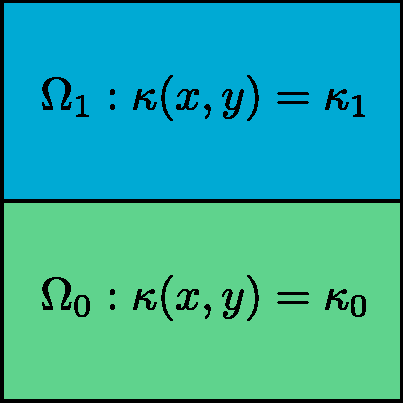
\includegraphics[width=0.5\linewidth]{fig/subdomains.pdf}}
 \caption{
 两个具有不同材料参数的子域。\label{fig:subdomains}
 }
\end{figure}

变分公式可以很容易地表达在FEniCS中
如下:
\begin{python}
a = kappa*dot(grad(u), grad(v))*dx
L = f*v*dx
\end{python}
在本节的其余部分,我们将讨论不同的策略
用于将系数\texttt{kappa}定义为需要的\texttt{Expression}
两个子域中的值不同。

\subsection{使用表达式来定义子域}

实现可变系数的最简单的方法
$\kappa = \kappa(x,y)$是定义一个\texttt{Expression},它依赖于
坐标$x$和$y$。 我们以前用过\texttt{Expression}
类基于简单公式定义表达式。或者,
一个\texttt{Expression}可以被定义为一个允许更多的Python类
复杂的逻辑。 以下代码片段说明了这一点
施工:

\begin{python}
class K(Expression):
    def set_k_values(self, k_0, k_1):
        self.k_0, self.k_1 = k_0, k_1

    def eval(self, value, x):
        "Set value[0] to value at point x"
        tol = 1E-14
        if x[1] <= 0.5 + tol:
            value[0] = self.k_0
        else:
            value[0] = self.k_1

# Initialize kappa
kappa = K(degree=0)
kappa.set_k_values(1, 0.01)
\end{python}
\texttt{eval}方法在定义函数方面提供了很大的灵活性,但a
缺点是FEniCS将为Python中的每个节点\texttt{x}调用\texttt{eval}
这是一个缓慢的过程。

另一种方法是使用C++字符串表达式
以前看过,在FEniCS中效率更高。 这可以做到
使用内联如果测试:

\begin{python}
tol = 1E-14
k_0 = 1.0
k_1 = 0.01
kappa = Expression('x[1] <= 0.5 + tol ? k_0 : k_1', degree=0,
               tol=tol, k_0=k_0, k_1=k_1)
\end{python}

如果子域名定义变量系数的这种方法起作用
是可以用几何表达的简单形状
不平等。 但是,对于更复杂的子域,我们将需要
使用更一般的技术,我们将在下面看到。

\index{boundary specification (class)}

\subsection{使用网格函数来定义子域}

\index{boundary markers}
\index{MeshFunction@{\rm\texttt{MeshFunction}}}
\index{CellFunction@{\rm\texttt{CellFunction}}}
\index{FacetFunction@{\rm\texttt{FacetFunction}}}

现在我们将介绍如何指定子域$\Omega_0$和$\Omega_1$
使用更一般的技术。 这种技术涉及使用两种
在使用子域时,FEniCS中必不可少的课程:
\texttt{SubDomain}和\texttt{MeshFunction}。 考虑下面的定义
边界$x = 0$:

\begin{python}
def boundary(x, on_boundary):
    tol = 1E-14
    return on_boundary and near(x[0], 0, tol)
\end{python}
这个边界定义实际上是更通用的捷径
FEniCS概念\texttt{SubDomain}。 一个\texttt{SubDomain}是一个定义a的类
区域在空间(子域)的成员函数\texttt{inside}
它返回\texttt{True}属于子域的点
\texttt{False}对于不属于子域的点。 这是怎么回事
指定边界$x = 0$作为\texttt{SubDomain}:

\begin{python}
class Boundary(SubDomain):
    def inside(self, x, on_boundary):
        tol = 1E-14
        return on_boundary and near(x[0], 0, tol)

boundary = Boundary()
bc = DirichletBC(V, Constant(0), boundary)
\end{python}
我们注意到\texttt{Boundary}类的\texttt{inside}函数是
(几乎)与以前的边界定义相同
\texttt{boundary}功能。 技术上,我们的
类\texttt{Boundary}是一个
\emph{subclass}的FEniCS类\texttt{SubDomain}。

我们将使用两个\texttt{SubDomain}子类来定义两个子域
$\Omega_0$和$\Omega_1$:

\begin{python}
tol = 1E-14

class Omega_0(SubDomain):
    def inside(self, x, on_boundary):
        return x[1] <= 0.5 + tol

class Omega_1(SubDomain):
    def inside(self, x, on_boundary):
        return x[1] >= 0.5 - tol
\end{python}
请注意在两个测试中使用\texttt{<=}和\texttt{> =}。 FEniCS会打电话给
\texttt{inside}函数为单元格中的每个顶点确定是否
不是该单元属于特定的子域。 因此,它是
重要的是,测试对于与对齐的单元格中的所有顶点保持一致
边界。 另外,我们使用宽容来确保
内部边界上的顶点$y = 0.5$将属于两者
子域。 这是一个有点反直觉,但是是必要的
使内部边界以上和下方的细胞属于
$\Omega_0$或$\Omega_1$。

要定义变量系数$\kappa$,我们将使用一个强大的工具
FEniCS称为\texttt{MeshFunction}。 一个\texttt{MeshFunction}是一个离散的
函数可以在一组所谓的网格中进行评估
实体。 FEniCS中的网格实体是顶点,边缘,
面或细胞(三角形或四面体)。 一个\texttt{MeshFunction}在单元格上
适合代表子域(材料),而a
\texttt{MeshFunction}超过面(边或面)用于表示
外部或内部边界。 一个\texttt{MeshFunction}在单元格上
也可用于表示网格细化的边界标记。 一个
FEniCS \texttt{MeshFunction}对其数据类型(如
整数或布尔值)及其维数(0 =顶点,1 =边
等等。)。 特殊子类\texttt{VertexFunction},\texttt{EdgeFunction}等等
提供了一个特定的\texttt{MeshFunction}的容易定义
尺寸。

由于在本示例中我们需要定义$\Omega$的子域,
我们使用\texttt{CellFunction}。 构造函数
给出两个参数:(1)值的类型:\texttt{'int'}用于整数,
\verb!'size_t'! 对于非负(无符号)整数,\texttt{'double'}为真
数字和\texttt{'bool'}用于逻辑值;(2)一个\texttt{Mesh}对象。
或者,构造函数只能使用一个文件名并进行初始化
\texttt{CellFunction}从文件中的数据。

我们首先创建一个非负的\texttt{CellFunction}
整数值(\verb!'size_t'!):

\begin{python}
materials = CellFunction('size_t', mesh)
\end{python}

接下来,我们使用两个子域来\emph{mark}属于每个的单元格
子域名:
\begin{python}
subdomain_0 = Omega_0()
subdomain_1 = Omega_1()
subdomain_0.mark(materials, 0)
subdomain_1.mark(materials, 1)
\end{python}

这将将网格函数\texttt{materials}的值设置为$0$
属于所有单元格的每个单元格属于$\Omega_0$和$1$
$\Omega_1$。 或者,我们可以使用以下等效代码
标记单元格:

\begin{python}
materials.set_all(0)
subdomain_1.mark(materials, 1)
\end{python}
检查网格函数的值,看到我们确实
正确定义了我们的子域,我们可以简单地绘制网格
功能:

\begin{python}
plot(materials, interactive=True)
\end{python}
我们也可能希望以后存储网格功能的值
使用:
\begin{python}
File('materials.xml.gz') << materials
\end{python}
这可以稍后从文件中读取如下:
\begin{python}
File('materials.xml.gz') >> materials
\end{python}

现在,使用网格函数\texttt{materials}的值来定义
可变系数$\kappa$,我们创建一个FEniCS \texttt{Expression}:

\begin{python}
class K(Expression):
    def __init__(self, materials, k_0, k_1, **kwargs):
        self.materials = materials
        self.k_0 = k_0
        self.k_1 = k_1

def eval_cell(self, values, x, cell):
        if self.materials[cell.index] == 0:
            values[0] = self.k_0
        else:
            values[0] = self.k_1

kappa = K(materials, k_0, k_1, degree=0)
\end{python}

这与我们上面定义的\texttt{Expression}子类似,但是我们
使用成员函数\verb!eval_cell! 代替常规
\texttt{eval}函数。 这个版本的评估功能有一个
附加\texttt{cell}参数,我们可以用来检查我们在哪个单元格
目前正在评估功能。 我们也定义了特殊的
功能\verb!__ init__! (构造函数),以便我们可以将所有数据传递给
\texttt{Expression}创建时。

由于我们使用几何测试来定义两个\texttt{SubDomains}
对于$\Omega_0$和$\Omega_1$,\texttt{MeshFunction}方法可能看起来像
使用简单方法的不必要的复杂性
\texttt{Expression}与if-test。 但是,一般的定义是
子域可能作为\texttt{MeshFunction}(从数据文件)可用,
可能生成的网格生成过程的一部分,而不是作为一个
简单的几何测试。 在这种情况下,这里所示的方法是
推荐使用子域名的方式。

\index{CompiledSubDomain@{\rm\texttt{CompiledSubDomain}}}

\subsection{使用C ++代码片段来定义子域}

\texttt{SubDomain}和\texttt{Expression} Python类非常方便,
但是它们的使用导致每个节点从C++到Python的函数调用
在网格中。 由于这涉及到巨大的成本,我们需要做出
如果性能是一个问题,使用C ++代码。

而不是在Python中编写\texttt{SubDomain}子类,我们可以改为使用
在FEniCS中使用\texttt{CompiledSubDomain}工具来指定C++中的子域
代码,从而加快我们的代码。 考虑
类的定义\verb!Omega_0! 和\verb!Omega_1! 以上在Python。该
定义这些子域的关键字符串可以用C++语法表示
并作为参数给出\texttt{CompiledSubDomain},如下所示:

\begin{python}
tol = 1E-14
subdomain_0 = CompiledSubDomain('x[1] <= 0.5 + tol', tol=tol)
subdomain_1 = CompiledSubDomain('x[1] >= 0.5 - tol', tol=tol)
\end{python}
如所见,可以使用关键字参数指定参数。
产生的对象,\verb!subdomain_0! 和\verb!subdomain_1!,可以使用
作为普通的\texttt{SubDomain}对象。

可以应用编译的子域字符串来指定边界
好:

\begin{python}
boundary_R = CompiledSubDomain('on_boundary && near(x[0], 1, tol)',
                               tol=1E-14)
\end{python}

也可以提供C++字符串(不带参数)
直接作为\texttt{DirichletBC}的第三个参数
构造一个\texttt{CompiledSubDomain}对象:

\begin{python}
bc1 = DirichletBC(V, value, 'on_boundary && near(x[0], 1, tol)')
\end{python}

Python \texttt{Expression}类也可以使用C ++重新定义更多
高效的代码。 再次考虑上面的class \texttt{K}的定义
对于变量系数$\kappa = \kappa(x)$。 这可以使用a重新定义
C++代码片段和关键字\texttt{cppcode}到常规FEniCS
\texttt{Expression}类:

\begin{python}
cppcode = """
class K : public Expression
{
public:

  void eval(Array<double>& values,
            const Array<double>& x,
            const ufc::cell& cell) const
  {
    if ((*materials)[cell.index] == 0)
      values[0] = k_0;
    else
      values[0] = k_1;
  }

  std::shared_ptr<MeshFunction<std::size_t>> materials;
  double k_0;
  double k_1;

};
"""

kappa = Expression(cppcode=cppcode, degree=0)
kappa.materials = materials
kappa.k_0 = k_0
kappa.k_1 = k_1
\end{python}

\section{设置多个Dirichlet,Neumann和Robin条件}
\label{ch:poisson0:multi:bc}
\index{Dirichlet boundary condition}
\index{Neumann boundary condition}
\index{Robin boundary condition}
\index{boundary conditions}

再次考虑可变系数Poisson问题
从部分~\ref{ftut:possion:2D:2mat:impl}。 我们现在讨论一下
如何实现边界条件的一般组合
Dirichlet,Neumann和Robin类型的这个模型问题。

\subsection{三种边界条件}

我们将我们的边界条件扩展到三种类型:
Dirichlet,Neumann和Robin。 Dirichlet条件适用于某些
部分$\GD^0, \GD^1,\ldots$,的边界:

\[ u = \ub^0\hbox{ on }\GD^0,\quad
u = \ub^1\hbox{ on }\GD^1, \quad \ldots,\]
其中$\ub^i$是规定的函数,$i=0,1, \ldots$。
在其他部分,$\GN^0, \GN^1, \ldots$,我们有
Neumann条件:

\[ -\kappa{\partial u\over\partial n} = g_{0}\hbox{ on }\GN^0,\quad
-\kappa{\partial u\over\partial n} = g_{1}\hbox{ on }\GN^1,\quad \ldots,
\]
最后,我们有\emph{Robin条件}:

\begin{equation*}
-\kappa{\partial u\over\partial n} = r(u-s),
\label{ch:poisson0:multi:bc:Robin}
\end{equation*}
其中$r$和$s$是指定的函数。 Robin条件是
最常用于将热量传递给周围环境并产生
自然是从Newton的冷静法。 在这种情况下,$r$是一个热量
传递系数,$s$是温度
环境。 两者都可以是空间和时间依赖的。
Robin条件适用
在某些部分$\GR^0, \GR^1, \ldots$,的边界:

\[ -\kappa{\partial u\over\partial n} = r_0(u-s_0)\hbox{ on }\GR^0,\quad
-\kappa{\partial u\over\partial n} = r_1(u-s_1)\hbox{ on }\GR^1,\quad \ldots
\]

\subsection{PDE问题}

用上面的符号,模型问题要用多个解决
Dirichlet,Neumann和Robin条件可以表达如下:

\begin{alignat}{2}
-\nabla\cdot(\kappa\nabla u) &= f \quad&&\mbox{in } \Omega, \label{ch:poisson0:2D:DN3}\\
u &= \ub^i &&\mbox{on } \GD^i,\quad i=0,1,\ldots
\label{ch:poisson0:2D:DN3:bcD}\\
-\kappa{\partial u\over\partial n} &= g_i &&\mbox{on } \GN^i,\quad
i=0,1,\ldots
\label{ch:poisson0:2D:DN3:bcN}\\
-\kappa{\partial u\over\partial n} &= r_i(u-s_i) \quad&&\mbox{on } \GR^i,\quad
i=0,1,\ldots
\label{ch:poisson0:2D:DN3:bcR}
\end{alignat}

\subsection{变化公式}

像往常一样,我们乘以一个测试函数$v$并按部分进行集成:

\begin{equation*}
 -\int_\Omega \nabla\cdot(\kappa\nabla u) v \dx
= \int_\Omega \kappa\nabla u\cdot \nabla v \dx -
\int_{\partial\Omega}\kappa\frac{\partial u}{\partial n}v \ds\tp
\end{equation*}
在边界的Dirichlet部分($\GD^i$),边界积分
$v = 0$以后消失。 在边界的剩余部分,我们
将边界积分分解为Neumann部分的贡献
($\GN^i$)和Robin部分($\GR^i$)。 插入边界条件,
我们获得

\begin{align*}
-\int_{\partial\Omega} \kappa\frac{\partial u}{\partial n}v \ds
&=
-\sum_i\int_{\GN^i} \kappa\frac{\partial u}{\partial n} \ds
-\sum_i\int_{\GR^i} \kappa\frac{\partial u}{\partial n} \ds\\
&=
\sum_i\int_{\GN^i}g_i \ds +
\sum_i\int_{\GR^i}r_i(u-s_i) \ds\tp
\end{align*}
因此,我们得到以下变分问题:

\begin{equation}
F = \int_{\Omega} \kappa\nabla u\cdot \nabla v \dx +
\sum_i\int_{\GN^i} g_iv \ds +
\sum_i\int_{\GR^i}r_i(u-s_i)v \ds
- \int_{\Omega} fv \dx =0\tp
\label{ch:poisson0:multi:bc:varform}
\end{equation}

我们已经习惯了在这个写作中写出这种变异形式
标准符号$a(u,v)= L(v)$,这要求我们识别所有
积分取决于试验功能$u$,并收集这些
$a(u,v)$,而剩余的积分则为$L(v)$。 积分
由于Robin条件必须分为两部分:

\begin{equation*}
\int_{\GR^i}r_i(u-s_i)v \ds
= \int_{\GR^i} r_iuv \ds - \int_{\GR^i}r_is_iv \ds\tp
\end{equation*}
我们有

\begin{align}
a(u, v) &= \int_{\Omega} \kappa\nabla u\cdot \nabla v \dx
+ \sum_i\int_{\GR^i}r_iuv \ds,
\label{ch:poisson0:2D:DN3:var:a}\\
L(v) &= \int_{\Omega} fv \dx -
\sum_i\int_{\GN^i} g_i v \ds + \sum_i\int_{\GR^i}r_is_iv \ds\tp
\label{ch:poisson0:2D:DN3:var:L}
\end{align}
或者,我们可以保留配方
(\ref{ch:poisson0:multi:bc:varform}),并解决变分
作为FEniCS中的非线性问题(\texttt{F == 0})或使用FEniCS
函数\texttt{lhs}和\texttt{rhs}来提取双线性和线性部分
\texttt{F}:

\begin{python}
a = lhs(F)
L = rhs(F)
\end{python}
请注意,如果我们选择将该线性问题解决为非线性问题
问题,Newton迭代将在单次迭代中收敛。

\subsection{FEniCS实现}

让我们来看看如何扩展我们的Poisson求解器来处理一般
Dirichlet,Neumann和Robin边界条件的组合。
与以前的代码相比,我们必须考虑以下几点
扩展:

\begin{itemize}
  \item 定义边界不同部分的标记。

  \item 使用标记将边界积分成部分。
\end{itemize}

\noindent
第一个任务的一般方法是标记所需的每个
标记0,1,2等的边界部分。 在这里我们瞄准了
单位正方形的四边,标有0($x = 0$),1($x = 1$),2
($y = 0$)和3($y = 1$)。 标记将使用a定义
\texttt{MeshFunction},但与第~\ref{ftut:possion:2D:2mat:impl}相反,这不是单元格的一个功能,而是
一个超过网格面的功能。 我们使用\texttt{FacetFunction}
这个目的:

\begin{python}
boundary_markers = FacetFunction('size_t', mesh)
\end{python}
如在~\ref{ftut:possion:2D:2mat:impl}中,我们使用一个子类
\texttt{SubDomain}来标识网格的各个部分
功能。 可能设置更复杂几何域的域的问题
用于将边界标记为网格的一部分的网格功能
代。 在我们的例子中,可以标记边界$x = 0$
如下:

\begin{python}
class BoundaryX0(SubDomain):
    tol = 1E-14
    def inside(self, x, on_boundary):
        return on_boundary and near(x[0], 0, tol)

bx0 = BoundaryX0()
bx0.mark(boundary_markers, 0)
\end{python}
类似地,我们创建类\texttt{BoundaryX1}($x = 1$),\texttt{BoundaryY0}
($y = 0$)和\texttt{BoundaryY1}($y = 1$)边界,并将其标记为
子域1,2和3。

为了实现的一般性,我们让用户指定
什么样的边界条件适用于四个中的每一个
边界。 为此,我们设置了一个Python字典
键作为子域号,值作为字典指定
关键的条件和作为其价值的功能。
例如,

\begin{python}
boundary_conditions = {0: {'Dirichlet': u_D},
                       1: {'Robin':     (r, s)},
                       2: {'Neumann':   g},
                       3: {'Neumann',   0}}
\end{python}
指定

\begin{itemize}
 \item 一个Dirichlet条件 $u = \ub$ 对于 $x = 0$;

 \item 一个Robin条件 $-\kappa\partial_n u = r(u-s)$ 对于 $x = 1$;

 \item 一个Neumann条件 $-\kappa\partial_n u = g$ 对于 $y = 0$;

 \item 一个Neumann条件 $-\kappa\partial_n u = 0$ 对于 $y = 1$.
\end{itemize}

\noindent
如在~\ref{ch:poisson0:multiple:Dirichlet}中所述的多个
Dirichlet条件必须收集在\texttt{DirichletBC}的列表中
对象。 基于\verb!boundary_conditions! 数据结构如上,我们
可以通过以下代码片段构建此列表:

\begin{python}
bcs = []
for i in boundary_conditions:
    if 'Dirichlet' in boundary_conditions[i]:
        bc = DirichletBC(V, boundary_conditions[i]['Dirichlet'],
                         boundary_markers, i)
        bcs.append(bc)
\end{python}

变分问题的一个新方面是两个不同的
边界积分超过$\GN^i$和$\GR^i$。
在外部细胞方面有一个网格功能(我们的
\verb!boundary_markers! 对象),子域(边界部分)
编号为$0,1,2,\ldots$,特殊符号\texttt{ds(0)}
意味着在子域(部分)0,\texttt{ds(1)}表示的集成
整合子域(部分)1,依此类推。
多个\texttt{ds}类型对象的想法概括为卷
积分:\texttt{dx(0)},\texttt{dx(1)}等,用于
在$\Omega$内的子域0,1等集成。

为了使用\texttt{ds(i)}在边界部分表达积分,我们必须
首先根据边界标记重新定义度量\texttt{ds}:

\begin{python}
ds = Measure('ds', domain=mesh, subdomain_data=boundary_markers)
\end{python}
同样,如果我们想要在域的不同部分进行集成,
我们将\texttt{dx}重新定义为

\begin{python}
dx = Measure('dx', domain=mesh, subdomain_data=domain_markers)
\end{python}
\verb!domain_markers! 是\texttt{CellFunction}定义$\Omega$中的子域名。

假设我们在子域上具有值为\texttt{r}和\texttt{s}的Robin条件
\texttt{R},在子域\texttt{N}上的值为\texttt{g}的Neumann条件。该
然后可以写出变化形式

\begin{python}
a = kappa*dot(grad(u), grad(v))*dx + r*u*v*ds(R)
L = f*v*dx - g*v*ds(N) + r*s*v*ds(R)
\end{python}

在我们的情况下,事情变得复杂了一些
关于Neumann和Robin条件的积分的信息
在 \\
\verb!boundary_conditions! 数据结构。 我们可以收集
所有Neumann条件由以下代码片段:

\begin{python}
integrals_N = []
for i in boundary_conditions:
    if 'Neumann' in boundary_conditions[i]:
        if boundary_conditions[i]['Neumann'] != 0:
            g = boundary_conditions[i]['Neumann']
            integrals_N.append(g*v*ds(i))
\end{python}
应用\verb!sum(integrals_N)! 将\texttt{+}运算符应用到
变体形式在\verb!integrals_N! 列表和结果
在积分中,我们需要右边的\texttt{L}
变化形式。

Robin条件的积分可以同样收集
列表中:

\begin{python}
integrals_R_a = []
integrals_R_L = []
for i in boundary_conditions:
    if 'Robin' in boundary_conditions[i]:
        r, s = boundary_conditions[i]['Robin']
        integrals_R_a.append(r*u*v*ds(i))
        integrals_R_L.append(r*s*v*ds(i))
\end{python}

我们现在可以定义\texttt{a}和\texttt{L}表达式
在变分公式中:

\begin{python}
a = kappa*dot(grad(u), grad(v))*dx + sum(integrals_R_a)
L = f*v*dx - sum(integrals_N) + sum(integrals_R_L)
\end{python}

\index{lhs@{\rm\texttt{lhs}}}
\index{rhs@{\rm\texttt{rhs}}}

或者,我们可以使用FEniCS函数\texttt{lhs}和\texttt{rhs}作为
以简化Robin的术语提取
积分:

\begin{python}
integrals_R = []
for i in boundary_conditions:
    if 'Robin' in boundary_conditions[i]:
        r, s = boundary_conditions[i]['Robin']
        integrals_R.append(r*(u - s)*v*ds(i))

F = kappa*dot(grad(u), grad(v))*dx + \
    sum(integrals_R) - f*v*dx + sum(integrals_N)
a, L = lhs(F), rhs(F)
\end{python}
这一次,我们可以更自然地定义积分
Robin条件为\texttt{r*(u - s)*v*ds(i)}。

完整的代码可以在函数中找到
\verb!solver_bcs! 在程序中
\begin{center}
\url{https://fenicsproject.org/pub/tutorial/python/vol1/ft10_poisson_extended.py}。
\end{center}
\index{ft10\_poisson\_extended.py@{\rm\texttt{ft10\_poisson\_extended.py}}}

\subsection{测试问题}

我们将使用相同的确切解决方案$\uex = 1 + x^2 + 2y^2$,如“~\ref{ch:fundamentals}”所示,因此需要$\kappa = 1$和$f = -6$。 我们的域名
是单位平方,我们将Dirichlet条件分配给$x = 0$和
$x = 1$,$y = 0$的Robin条件,以及Neumann条件
$y =1$。 给定的确切解决方案$\uex$,我们意识到
$y = 1$的Neumann条件是
$-\partial u / \partial n = -\partial u /\partial y = 4y = 4$,
而可以选择$y = 0$的Robin条件
很多方法。 由于$-\partial u/\partial n=\partial u/\partial y = 0$ at
$y = 0$,我们可以选择$s = \uex$并指定$r \neq 0$
Robin条件。 我们将设置$r = 1000$和$s = \uex$。

因此边界部分$\GD^0$: $x=0$, $\GD^1$: $x=1$,
$\GR^0$: $y=0$, 和 $\GN^0$: $y=1$。

在实施这个测试问题时,尤其是其他测试
使用更复杂的表达式的问题,有利于使用
符号计算。 下面我们将确切的解决方案定义为\texttt{sympy}
表达并从他们的数学派生其他功能
定义。 然后我们将这些表达式转换成C/C++代码,
然后可以用来定义\texttt{Expression}对象。

\begin{python}
# Define manufactured solution in sympy and derive f, g, etc.
import sympy as sym
x, y = sym.symbols('x[0], x[1]')            # needed by UFL
u = 1 + x**2 + 2*y**2                       # exact solution
u_e = u                                     # exact solution
u_00 = u.subs(x, 0)                         # restrict to x = 0
u_01 = u.subs(x, 1)                         # restrict to x = 1
f = -sym.diff(u, x, 2) - sym.diff(u, y, 2)  # -Laplace(u)
f = sym.simplify(f)                         # simplify f
g = -sym.diff(u, y).subs(y, 1)              # compute g = -du/dn
r = 1000                                    # Robin data, arbitrary
s = u                                       # Robin data, u = s

# Collect variables
variables = [u_e, u_00, u_01, f, g, r, s]

# Turn into C/C++ code strings
variables = [sym.printing.ccode(var) for var in variables]

# Turn into FEniCS Expressions
variables = [Expression(var, degree=2) for var in variables]

# Extract variables
u_e, u_00, u_01, f, g, r, s = variables

# Define boundary conditions
boundary_conditions = {0: {'Dirichlet': u_00},   # x = 0
                       1: {'Dirichlet': u_01},   # x = 1
                       2: {'Robin':     (r, s)}, # y = 0
                       3: {'Neumann':   g}}      # y = 1
\end{python}

完整的代码可以在函数中找到
\verb!demo_bcs! 在程序中
\begin{center}
\url{https://fenicsproject.org/pub/tutorial/python/vol1/ft10_poisson_extended.py}。
\end{center}

\subsection{调试边界条件}

在执行许多问题时很容易犯错误
不同类型的边界条件,如本案。 一
调试边界条件的方法是遍历所有顶点
协调并检查\texttt{SubDomain.inside}方法是否标记
顶点在边界上。 另一个有用的方法是列出哪个
受Dirichlet条件影响的自由度
一级Lagrange($\mathsf{P} _1 $)元素,打印
对应的顶点坐标如下图所示
代码段:

\begin{python}
if debug1:

    # Print all vertices that belong to the boundary parts
    for x in mesh.coordinates():
        if bx0.inside(x, True): print('%s is on x = 0' % x)
        if bx1.inside(x, True): print('%s is on x = 1' % x)
        if by0.inside(x, True): print('%s is on y = 0' % x)
        if by1.inside(x, True): print('%s is on y = 1' % x)

    # Print the Dirichlet conditions
    print('Number of Dirichlet conditions:', len(bcs))
    if V.ufl_element().degree() == 1:  # P1 elements
        d2v = dof_to_vertex_map(V)
        coor = mesh.coordinates()
        for i, bc in enumerate(bcs):
            print('Dirichlet condition %d' % i)
            boundary_values = bc.get_boundary_values()
            for dof in boundary_values:
                print('   dof %2d: u = %g' % (dof, boundary_values[dof]))
                if V.ufl_element().degree() == 1:
                    print('    at point %s' %
                          (str(tuple(coor[d2v[dof]].tolist()))))
\end{python}

\begin{notice}[调用\texttt{inside}方法]
在上面的代码片段中,我们称之为每个的inside方法
网格的坐标。 我们也可以打印输出
\texttt{inside}方法。 那么这个方法就是令人惊讶的
不仅要求与自由度相关的要点。
对于$\mathsf{P}_1$元素,也为每个元素调用该方法
细胞每一面的中点。 这是因为Dirichlet
默认情况下,只有整个方面可以说是设置的
在限定边界的条件下。
\end{notice}

\section{用子域生成网格}

到目前为止,我们的工作主要是简单的网格(单位面积)和
根据简单的几何测试定义边界和子域
像$x = 0$或$y \leq 0.5$。 对于更复杂的几何,它不是
以这种方式指定边界和子域的现实。 代替,
边界和子域必须定义为网格的一部分
生成过程。 现在我们来看一下如何使用FEniCS网格
生成工具\texttt{mshr}以生成网格并定义子域。

\subsection{PDE问题}

\index{magnetostatics}
\index{Maxwell's equations}

我们将再次解决Poisson方程,但这次为a
不同的应用。 考虑一个带铜线的铁缸
如图~\ref{ftut1:fig:magnetostatics:geometry}围绕圆筒缠绕。 通过铜线a
静态电流$J = 1\,\mathrm{A}$正在流动,我们要计算
铁芯中的磁场$B$,铜线,和
周围的真空。

\begin{figure}[!ht]  % ftut1:fig:magnetostatics:geometry
 \centerline{
\includegraphics[width=0.5\linewidth]{fig/magnetostatics_geometry.pdf}}
 \caption{
 在圆柱体上缠绕铜线的铁芯横截面,这里以$n=8$的绕组。 内圆是铜线的横截面(“北”),外圆是铜线向下进入平面(“南”)的横截面。\label{ftut1:fig:magnetostatics:geometry}
 }
\end{figure}

首先,我们将问题简化为2D问题。 我们可以这样做
假设圆柱体沿着$z$ -axis和a延伸很远
后果是该领域几乎独立于
$Z$ - 协调。 接下来,我们考虑Maxwell的方程式得出a
磁场的Poisson方程(或其电位):

\begin{align}
  \nabla\cdot  D &= \varrho, \\
  \nabla\cdot  B &= 0, \\
  \nabla\times E &= -\frac{\partial B}{\partial t}, \\
  \nabla\times H &= \frac{\partial D}{\partial t} + J.
\end{align}
这里,$D$是位移场,$B$是磁性的
场,$E$是电场,$H$是磁场。 在
除了Maxwell方程之外,我们还需要一个本构关系
在$B$和$H$之间,

\begin{equation}
  B = \mu H,
\end{equation}
其适用于各向同性线性磁介质。 这里,$\mu$是
材料的磁导率。 现在,因为$B$是螺线管的
(不分散)根据Maxwell方程,我们知道$B$
必须是一些矢量字段$A$的卷曲。 这个字段叫做
磁矢量电位。 由于问题是静态的,因此
$\partial D/\partial t = 0$,就是这样

\begin{equation}
  J = \nabla \times H
    = \nabla \times (\mu^{-1} B)
    = \nabla \times (\mu^{-1} \nabla \times A)
    = -\nabla \cdot (\mu^{-1} \nabla A).
\end{equation}
在最后一步中,我们扩大了二次衍生品并使用了
量纲自由$A$简化方程式简单
磁矢量势的向量值Poisson问题; 如果
$B = \nabla \times A$,然后$B = \nabla \times (A + \nabla \psi)$
标量场$\psi$(量表功能)。 对于目前的问题,我们
因此需要解决以下2D Poisson问题
$z$-组件$A_z$的磁矢量电位:

\begin{align}
  - \nabla \cdot (\mu^{-1} \nabla A_z) &= J_z \quad \text{in } \Real^2, \\
  \lim_{|(x, y)| \rightarrow \infty} A_z &= 0.
\end{align}
由于我们无法在无限的域上解决这个问题,所以我们会
使用大型磁盘截断域,并设置$A_z = 0$
边界。 当前的$J_z$设置为$+1\,\mathrm{A}$在内部
一组圈(铜线横截面)和$-1\,\mathrm{A}$
图中的外部圆圈~\ref{ftut1:fig:magnetostatics:geometry}。

\index{infinite domain}

一旦计算了磁矢量电位,我们就可以
计算磁场$B = B(x,y)$

\begin{align}
  B(x, y) =
  \left(\frac{\partial A_z}{\partial y},
       -\frac{\partial A_z}{\partial x}\right).
\end{align}

\subsection{变化公式}

变分问题是通过乘以PDE得到的
具有$v$的测试函数,并以部件集成。 自边界
由于Dirichlet条件,积分消失,我们得到

\begin{equation}
  \int_{\Omega} \mu^{-1} \nabla A_z \cdot \nabla v \dx
  = \int_{\Omega} J_z v \dx,
\end{equation}
或者换句话说,$a(A_z,v) = L(v)$同

\begin{align}
  a(A_z, v) &= \int_{\Omega} \mu^{-1} \nabla A_z \cdot \nabla v \dx, \\
  L(v) &= \int_{\Omega} J_z v \dx.
\end{align}

\subsection{FEniCS实现}

第一步是为几何描述生成一个网格
图~\ref{ftut1:fig:magnetostatics:geometry}。 我们让$a$和$b$成为
铁缸的内外半径,让$c_1$和$c_2$
是铜线的两个同心分布的半径
交叉区域。 此外,我们让$r$是铜的半径
线,$R$是我们域的半径,$n$是数
绕组(总共$2n$铜线截面)。 这个
几何可以很容易的用\texttt{mshr}和一点点描述
Python编程:

\index{mshr}
\index{Circle@{\rm\texttt{Circle}}}
\index{generate\_mesh@{\rm\texttt{generate\_mesh}}}
\index{mesh generation}

\begin{python}
# Define geometry for background
domain = Circle(Point(0, 0), R)

# Define geometry for iron cylinder
cylinder = Circle(Point(0, 0), b) - Circle(Point(0, 0), a)

# Define geometry for wires (N = North (up), S = South (down))
angles_N = [i*2*pi/n for i in range(n)]
angles_S = [(i + 0.5)*2*pi/n for i in range(n)]
wires_N = [Circle(Point(c_1*cos(v), c_1*sin(v)), r) for v in angles_N]
wires_S = [Circle(Point(c_2*cos(v), c_2*sin(v)), r) for v in angles_S]
\end{python}

我们生成的网格将是整个磁盘的网格
半径$R$,但我们需要网格生成来尊重内部
由铁缸和铜线限定的边界。 我们也
想要\texttt{mshr}标记子域,以便我们可以轻松指定
材料参数($\mu$)和电流。 为此,我们使用
\texttt{mshr}功能\verb!set_subdomain! 如下:

\begin{python}
# Set subdomain for iron cylinder
domain.set_subdomain(1, cylinder)

# Set subdomains for wires
for (i, wire) in enumerate(wires_N):
    domain.set_subdomain(2 + i, wire)
for (i, wire) in enumerate(wires_S):
    domain.set_subdomain(2 + n + i, wire)
\end{python}
一旦子域被创建,我们可以生成网格:

\begin{python}
mesh = generate_mesh(domain, 128)
\end{python}
网格的细节如图~\ref{ftut1:fig:magnetostatics:mesh}所示。

\begin{figure}[!ht]  % ftut1:fig:magnetostatics:mesh
 \centerline{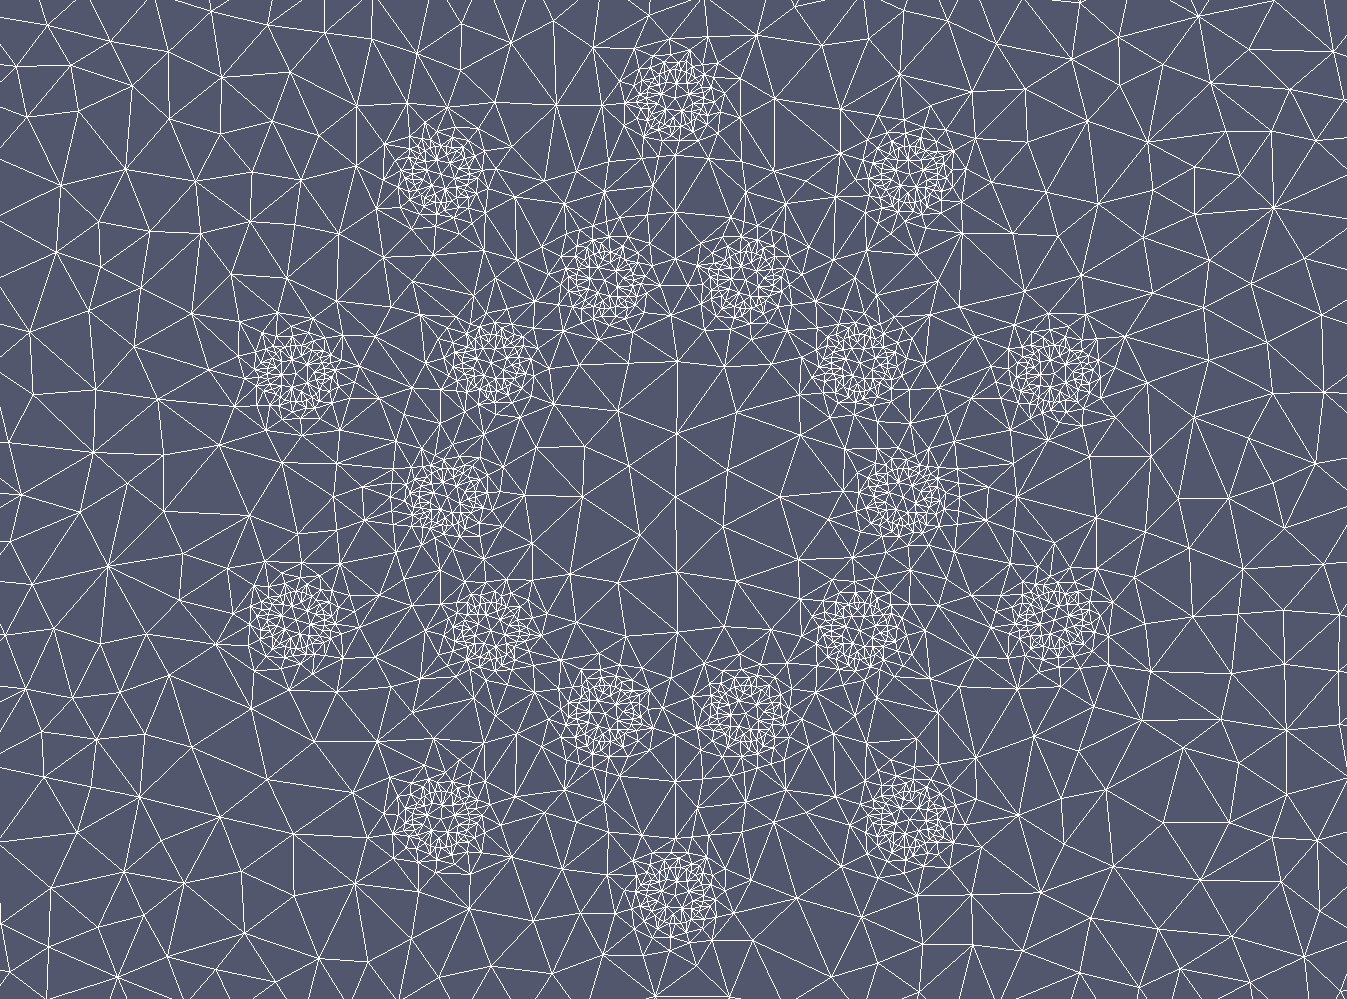
\includegraphics[width=0.95\linewidth]{fig/magnetostatics_mesh.png}}
 \caption{
 绘制(部分)为静磁测试问题产生的网格。 铁桶和铜线的子域清晰可见。\label{ftut1:fig:magnetostatics:mesh}
 }
\end{figure}

使用\texttt{mshr}生成的网格将包含有关的信息
我们定义的子域。 在定义中使用这些信息
我们的变分问题和子域依赖参数,我们将需要
创建一个标记子域的\texttt{MeshFunction}。 这可以很容易
通过调用成员函数\texttt{mesh.domains}创建的
\texttt{mshr}生成的子域数据:

\begin{python}
markers = MeshFunction('size_t', mesh, 2, mesh.domains())
\end{python}
该行用无符号整数值创建一个\texttt{MeshFunction}
子域号,其尺寸为2,其为单元格维度
这个2D问题。

我们现在可以像以前那样使用标记来重新定义
整合度量\texttt{dx}:

\index{Measure@{\rm\texttt{Measure}}}

\begin{python}
dx = Measure('dx', domain=mesh, subdomain_data=markers)
\end{python}
然后可以通过\texttt{dx(0)},\texttt{dx(1)}来表示子域上的积分,
等等。 我们用它来定义当前的$J_z = \pm 1\,\mathrm{A}$
在铜线上:

\begin{python}
J_N = Constant(1.0)
J_S = Constant(-1.0)
A_z = TrialFunction(V)
v = TestFunction(V)
a = (1 / mu)*dot(grad(A_z), grad(v))*dx
L_N = sum(J_N*v*dx(i) for i in range(2, 2 + n))
L_S = sum(J_S*v*dx(i) for i in range(2 + n, 2 + 2*n))
L = L_N + L_S
\end{python}

Permeability被定义为取决于该文件的\texttt{Expression}
子域号:
\begin{python}
class Permeability(Expression):
    def __init__(self, markers, **kwargs):
        self.markers = markers
    def eval_cell(self, values, x, cell):
        if self.markers[cell.index] == 0:
            values[0] = 4*pi*1e-7 # vacuum
        elif self.markers[cell.index] == 1:
            values[0] = 1e-5      # iron (should really be 6.3e-3)
        else:
            values[0] = 1.26e-6   # copper

mu = Permeability(markers, degree=1)
\end{python}
从这段代码片段可以看出,我们使用的是一个稍微不那么的极端
铁的磁导率值。 这是做的
解决方案有点有趣。 否则将是完全的
以铁缸为主。

最后,当计算$A_z$时,我们可以计算磁性
领域:

\begin{python}
W = VectorFunctionSpace(mesh, 'P', 1)
B = project(as_vector((A_z.dx(1), -A_z.dx(0))), W)
\end{python}
我们使用\verb!as_vector! 解释
\verb!(A_z.dx(1),-A_z.dx(0))! 作为UFL意义上的向量
形式语言,而不是Python元组。 所得的地块
磁矢量电位和磁场如图~\ref{ftut1:fig:magnetostatics:potential}
和~\ref{ftut1:fig:magnetostatics:field}所示。

\begin{figure}[!ht]  % ftut1:fig:magnetostatics:potential
 \centerline{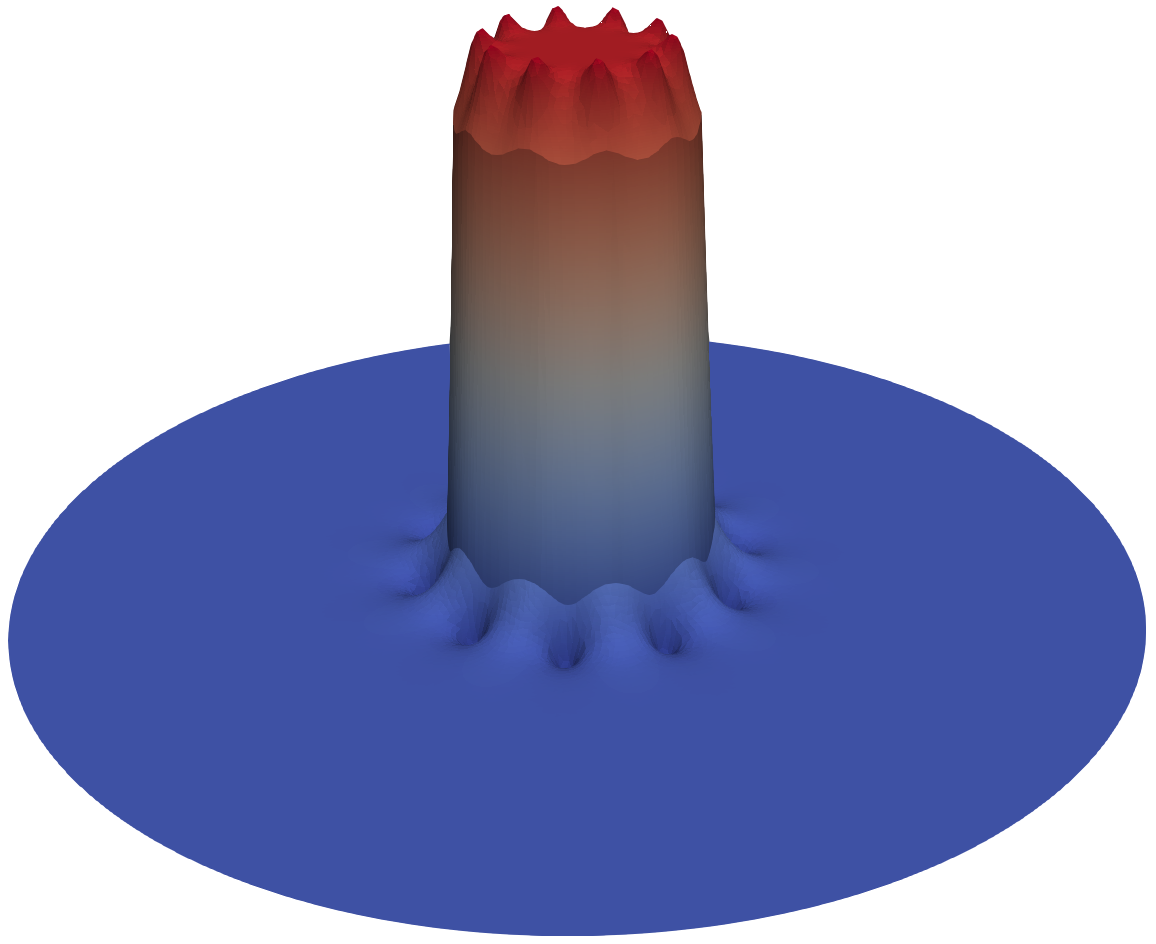
\includegraphics[width=0.95\linewidth]{fig/magnetostatics_potential.png}}
 \caption{
 剧情$z$元素$A_z$的磁矢量势。\label{ftut1:fig:magnetostatics:potential}
 }
\end{figure}

\begin{figure}[!ht]  % ftut1:fig:magnetostatics:field
 \centerline{
\includegraphics[width=0.75\linewidth]{fig/magnetostatics_field.png}}
 \caption{
 在$xy$平面上绘制磁场$B$。\label{ftut1:fig:magnetostatics:field}
 }
\end{figure}

计算磁场的完整代码如下。

\begin{python}
from fenics import *
from mshr import *
from math import sin, cos, pi

a = 1.0   # inner radius of iron cylinder
b = 1.2   # outer radius of iron cylinder
c_1 = 0.8 # radius for inner circle of copper wires
c_2 = 1.4 # radius for outer circle of copper wires
r = 0.1   # radius of copper wires
R = 5.0   # radius of domain
n = 10    # number of windings

# Define geometry for background
domain = Circle(Point(0, 0), R)

# Define geometry for iron cylinder
cylinder = Circle(Point(0, 0), b) - Circle(Point(0, 0), a)

# Define geometry for wires (N = North (up), S = South (down))
angles_N = [i*2*pi/n for i in range(n)]
angles_S = [(i + 0.5)*2*pi/n for i in range(n)]
wires_N = [Circle(Point(c_1*cos(v), c_1*sin(v)), r) for v in angles_N]
wires_S = [Circle(Point(c_2*cos(v), c_2*sin(v)), r) for v in angles_S]

# Set subdomain for iron cylinder
domain.set_subdomain(1, cylinder)

# Set subdomains for wires
for (i, wire) in enumerate(wires_N):
    domain.set_subdomain(2 + i, wire)
for (i, wire) in enumerate(wires_S):
    domain.set_subdomain(2 + n + i, wire)

# Create mesh
mesh = generate_mesh(domain, 32)

# Define function space
V = FunctionSpace(mesh, 'P', 1)

# Define boundary condition
bc = DirichletBC(V, Constant(0), 'on_boundary')

# Define subdomain markers and integration measure
markers = MeshFunction('size_t', mesh, 2, mesh.domains())
dx = Measure('dx', domain=mesh, subdomain_data=markers)

# Define current densities
J_N = Constant(1.0)
J_S = Constant(-1.0)

# Define magnetic permeability
class Permeability(Expression):
    def __init__(self, markers, **kwargs):
        self.markers = markers
    def eval_cell(self, values, x, cell):
        if self.markers[cell.index] == 0:
            values[0] = 4*pi*1e-7 # vacuum
        elif self.markers[cell.index] == 1:
            values[0] = 1e-5      # iron (should really be 6.3e-3)
        else:
            values[0] = 1.26e-6   # copper

mu = Permeability(markers, degree=1)

# Define variational problem
A_z = TrialFunction(V)
v = TestFunction(V)
a = (1 / mu)*dot(grad(A_z), grad(v))*dx
L_N = sum(J_N*v*dx(i) for i in range(2, 2 + n))
L_S = sum(J_S*v*dx(i) for i in range(2 + n, 2 + 2*n))
L = L_N + L_S

# Solve variational problem
A_z = Function(V)
solve(a == L, A_z, bc)

# Compute magnetic field (B = curl A)
W = VectorFunctionSpace(mesh, 'P', 1)
B = project(as_vector((A_z.dx(1), -A_z.dx(0))), W)

# Plot solution
plot(A_z)
plot(B)

# Save solution to file
vtkfile_A_z = File('magnetostatics/potential.pvd')
vtkfile_B = File('magnetostatics/field.pvd')
vtkfile_A_z << A_z
vtkfile_B << B

# Hold plot
interactive()
\end{python}
该示例程序可以在文件中找到
\begin{center}
\url{https://fenicsproject.org/pub/tutorial/python/vol1/ft11_magnetostatics.py}。
\end{center}

\index{ft11\_magnetostatics.py@{\rm\texttt{ft11\_magnetostatics.py}}}
